%%%%%%%%%%%%
%
% $Autor: Wings $
% $Datum: 2019-03-05 08:03:15Z $
% $Pfad: TemplateSensor $
% $Version: 4250 $
% !TeX spellcheck = en_GB/de_DE
% !TeX encoding = utf8
% !TeX root = filename 
% !TeX TXS-program:bibliography = txs:///biber
%
%%%%%%%%%%%%

% Structure
\chapter{DC-Gleichstrommotor}


\section{Allgemeines}

General description

cite books

\section{Motraxx SR555SHP}

cite board

\section{Spezifikationen}

\begin{center}
	\begin{figure}
		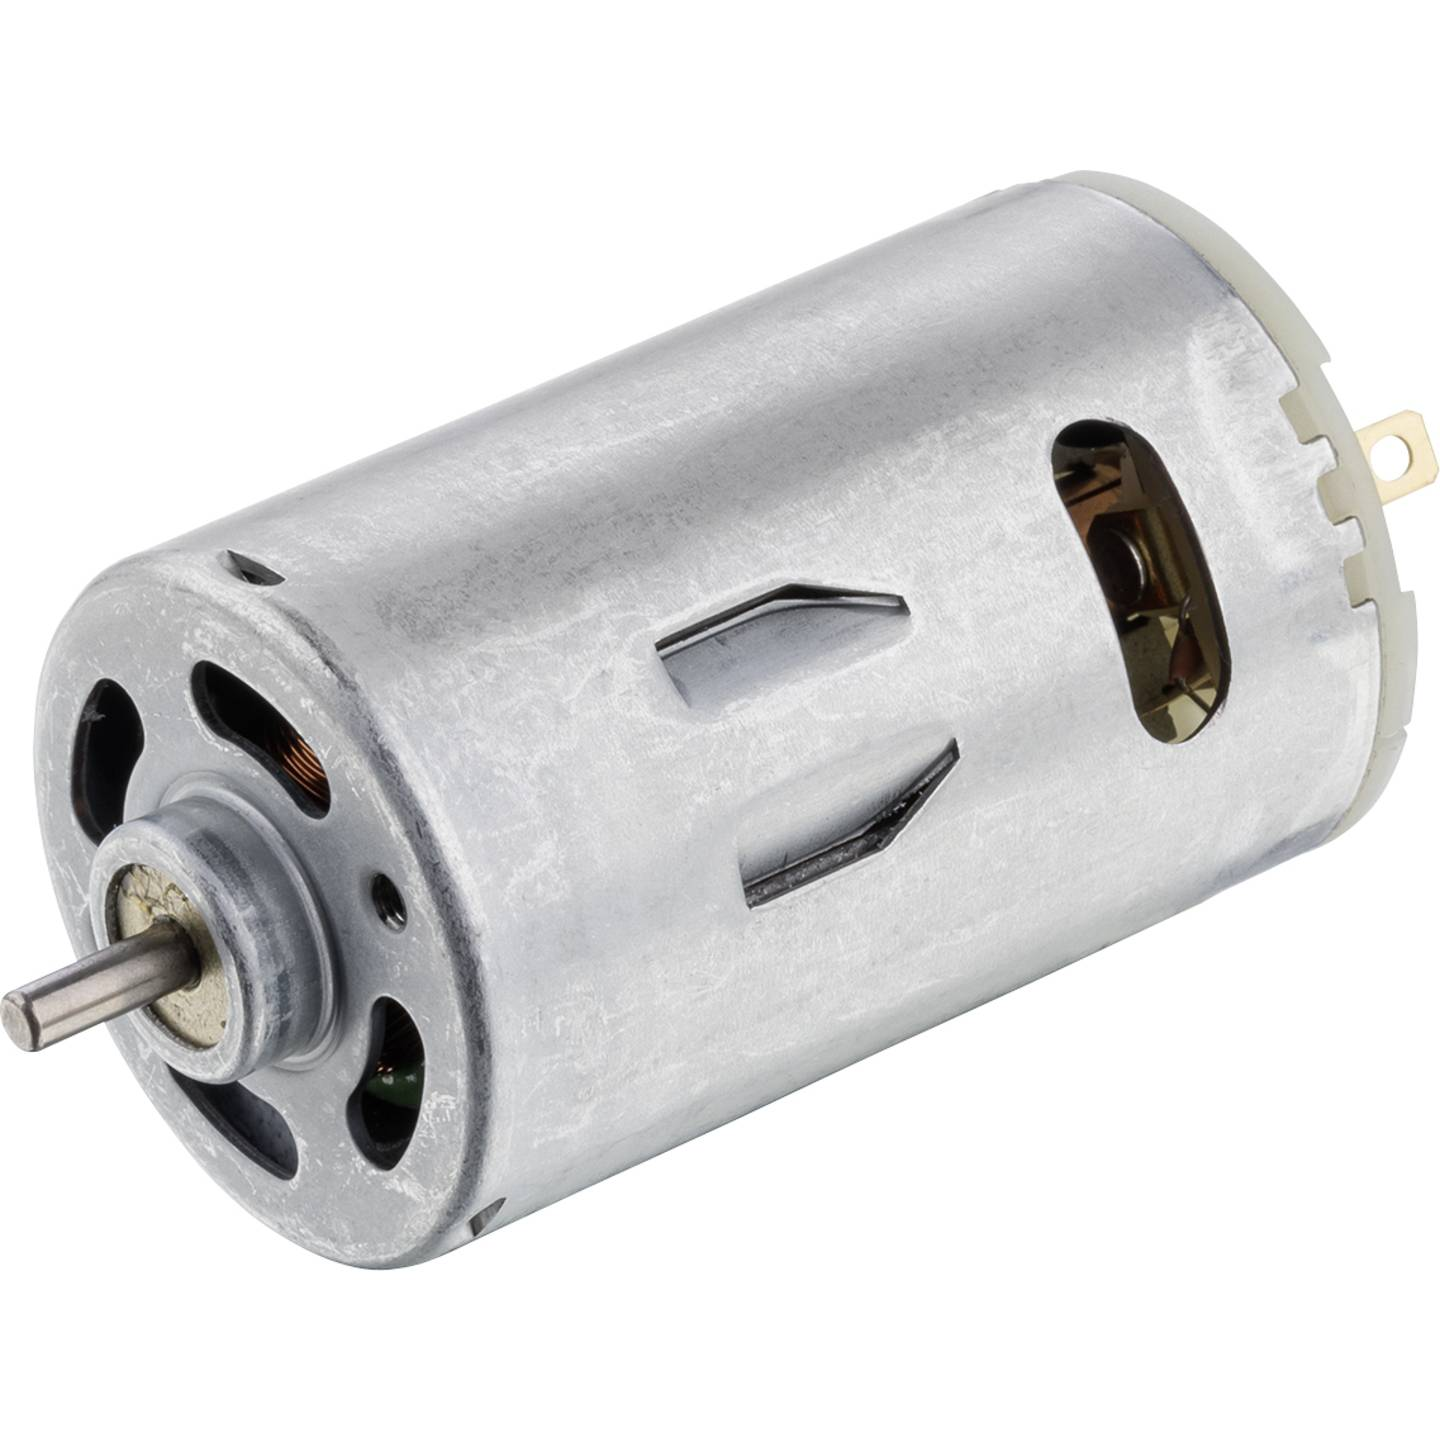
\includegraphics[scale=0.25]{../../Images/BOM/Motraxx_SR555SHP-3247S-75_Universal_Brushed_Elektromotor.jpg}
		\caption{Der Motor Motraxx SR555SHP nach (QUELLE)} 
		\label{pic:SR555SHP}
	\end{figure}
\end{center}

\begin{table}[h!]
	\caption{Spezifikationen des Motors (QUELLE)}
	\begin{center}
		\begin{tabular}{|l|l|}
			\hline
			\textbf{Parameter} &\textbf{Wert/Detail}\\
			\hline
			Modell & Motraxx SR555SHP\\
			\hline
			Typ  & DC-Gleichstrommotor\\
			\hline 
			Betriebsspannung & 10 bis 14 $V$ DC\\
			\hline 
			Nennspannung & 12 $V$ DC\\
			\hline
			Abgabeleistung & 13 $W$\\
			\hline
			Last-Drehzahl & 4800 $U/min$ \\
			\hline
			Max. Drehmoment & 25.18 $Nmm$\\
			\hline
			Anschlüsse & +V, -V\\ 
			\hline
			Wellen-Ø & 3.175 $mm$\\ 
			\hline
			Durchmesser & 37.5 $mm$\\ 
			\hline
			Länge & 57 $mm$\\ 
			\hline
			Gewicht & 224 $g$\\ 
			\hline
		\end{tabular}
		\label{TabelleSpezifikationMOT}
	\end{center}
\end{table} 


Der Motortreiber besitzt wie in \ref{pic:SR555SHP} erkenntlich zwei Anschlüsse. Diese Anschlüsse können wie folgt beschrieben werden: 
\begin{enumerate}
	\item \textbf{Leistungsanschlüsse}
	\begin{itemize}
		\item \textbf{+V}: Positiver Spannungsanschluss (10$-$14 $V$ DC)
		\item \textbf{-V}: Negativer Spannungsanschluss (Masse)
	\end{itemize}
\end{enumerate}



\section{Anwendungsbeispiel}
\label{sec:AnwendungSR555SHP}
Der Motor lässt sich mit kleinem Aufwand anschließen und verwenden. 
%Hier beschreibung

\begin{center}
	\begin{figure}
		\includegraphics[scale=0.35]{Bild Anschluss} %tikz oder bild noch erstellen
		\caption{Anschlussbeispiel des SR555SHP nach Quelle} 
		\label{pic:SR555SHPAnschluss} 
	\end{figure}
\end{center}



\subsection{Code}
Zum testen des Motraxx SR555SHP ist kein Mikrocontroller und somit auch kein Code notwendig.

\subsection{Einfacher Funktionstest}
Um die Ordnungsgemäße Funktion des Motors sicherzustellen, ist es sinnvoll ihn vor der Verwendung zu testen. Hierfür kann die in \ref{pic:SR555SHPAnschluss} gezeigte Schaltung verwendet werden. Um die Funktion des Motors zu prüfen kann folgendes Vorgehen befolgt werden: 

\begin{center}
	\begin{enumerate}
		\item Alle Anschlüsse und Verbindungen nach \ref{pic:SR555SHPAnschluss} verbinden und auf festen Sitz prüfen. 
		\item Spannungsversorgung (12V) einschalten.   
		\item Prüfen ob der Motor sich mit konstanter Drehzahl dreht. 
	\end{enumerate}  
\end{center}

Sollte sich der Motor nicht drehen oder unregelmäßig laufen, so sollten zunächst alle Verbindungen auf korrekten Anschluss sowie festen Sitz überprüft werden. Ein Austausch der Steckverbindungsleitungen kann zudem Kabelbrüche als mögliche Fehlerursache ausschließen.
Eine Kalibrierung des Motors im klassischen Sinne ist nicht möglich. Dennoch kann es sinnvoll sein, die Last-Drehzahl von 4800 $U/min$ zu überprüfen, um möglichen Verschleiß oder Reibung 



\section{weiterführende Literatur} 
\begin{center}
	\begin{enumerate}
		
	%Hier Literatur anfügen
	
	\end{enumerate}
\end{center}
